\setcounter{section}{4}
\setcounter{subsection}{4}
\setcounter{subsubsection}{2}
\setcounter{equation}{29}

\subsubsection{Mehratomige Moleküle und ihre Rotationsspektren}
	Wesentlich zur Beschreibung der Rotationsspektren sind die drei Hauptträgheitsmomente: $ \Theta_{\mathrm{A}}$, $ \Theta_{\mathrm{B}}$, $ \Theta_{\mathrm{C}}$. Symmetrieachsen sind Hauptträgheitsachsen.\\

	\begin{figure}[H]
			\centering
			\includegraphics[width=0.25\textwidth]{./figures/VL09_Abbildung_1.tikz}
			\caption{Das Tetrachlormethan \ce{CCl4} bildet einen deformierten Tetraeder. Wegen der Hauptträgheitsmomente $\Theta_\text A = \Theta_\mathrm B \neq \Theta_\mathrm C$ wird es als {symmetrischer Kreisel} bezeichnet.}
			\label{fig:vl09_tetrachlormethan}
	\end{figure}

	Man unterscheidet zwischen dem
	\begin{itemize}
		\item {Unsymmetrischen Kreisel}, bei dem alle drei Hauptträgheitsachsen verschieden sind;
		\item {Symmetrischen Kreisel}, bei dem zwei der drei Hauptträgheitsmomente gleich sind, bspw. \ce{CH3Cl}, \ce{NH3};
		\item {Kugelkreisel}, bei dem alle drei Hauptträgheitsmomente gleich sind, bspw. \ce{CCl4}, \ce{CH4}.
	\end{itemize}

Die Berechnung der Rotationsenergien benötigt eine quantenmechanische Behandlung (siehe Haken-Wolf, Kapitel 11.2).

\subsubsection{Anwendung der Molekülrotation}
	Ein weit bekannter Anwendungsfall der Molekülrotation ist die Mikrowelle, in welcher \ce{H2O}-Moleküle bei $ \nu = \SI{2,45}{\giga \hertz}$ ($ \lambda \sim \SI{12}{\centi \meter}$) zur Rotation angeregt werden. Die dielektrische Relaxation erwärmt hierbei das Präparat weiter (vertiefendes Lesen: Physik Journal 11/2005).\\

	Eine weitere interessante Anwendung findet sich in der Radiowellen-Astrophysik. Dabei werden über die Emission von Rotationsspektren verschiedene Moleküle im Universum identifiziert, wie z.B. \ce{H2O}, Ammoniak, Formaldehyd, Methanol etc. Die Suche nach diesen Molekülen geht direkt einher mit der Suche nach fremden Leben.

\subsection{Schwingungsspektren von Molekülen}
	Schwingungen geben grundlegende Auskunft über die Kopplungen der verschiedenen Atome. \autoref{fig:vl09_abbildung_2} zeigt einen schematischen Versuchsaufbau zur Messung der Schwingungsspektren eines Moleküls.\\

	\begin{figure}[H]
		\centering
		\incfig{vl09_abbildung_2}
		\caption{Schematischer Versuchsaufbau zur Messung von Schwingungsspektren.}
		\label{fig:vl09_abbildung_2}
	\end{figure}

	Zu den Licht-/Laserquellen, die bei der Spektroskopie angewendet werden, gehören thermische Strahler wie der Nernst-Stift, Gaslampen wie Quecksilber oder \ce{Xe}-Hochdrucklampen und Quantenkaskadenlaser. Nachdem das Licht das Präparat passiert hat, gelangt es entweder ins Gitter- oder Fourierspektrometer, welches entweder eine Photodiode oder ein Bolometer als Detektor besitzt.

	\subsubsection{Zweiatomige Moleküle, harmonische Näherung}
	Ein zweiatomiges Molekül wird als Federpendel mit Feder $k$ zwischen den Atomen genähert, vgl. \autoref{fig:vl09_federmodell}.
	\begin{figure}[H]
			\centering
			\includegraphics[width=0.25\textwidth]{./figures/VL09_Abbildung_3.tikz}
			\caption{Näherung der Molekülschwingung als Federpendel zwischen den Atomen.}
			\label{fig:vl09_federmodell}
	\end{figure}
	Verwendet wird das harmonische Parabelpotential
	\begin{equation}
		\label{4.30}
		V = \frac{1}{2} K \left( R-R_{\mathrm{e}} \right) ^2
	\end{equation}
	mit der Eigenfrequenz
	$$
	\omega_{\mathrm{e}} = \sqrt{ \frac{K}{m_{ \nu}}}.
	$$ 
	Die Schwingungsenergie beträgt dann
	\begin{important}
		\begin{equation}
			\label{4.31}
			E_{\text{vib}} = \hbar \omega_{\mathrm{e}} \left( \nu +\frac{1}{2} \right) \quad \text{mit}\quad \nu = 0,1,2,3\ldots
		\end{equation}
	\end{important}

	\begin{definition}{}
		Zur Betrachtung mit Wellenzahlen in \unit{\per\centi\meter} wird 
		\begin{equation}
			\label{4.32}
			G_{ \nu}= \frac{ E_{\text{vib}}}{\mathrm{h} \mathrm{c}} = \overline{ \nu}_{\mathrm{e}} \left( \nu + \frac{1}{2} \right) 
		\end{equation}
		definiert mit der Schwingungskonstante $\overline\nu_\mathrm e$. 
	\end{definition}


	Die Auswahlregel für Übergänge ist $ \Delta \nu = \pm 1$. Ein Übergang ist erlaubt, wenn mit der Schwingung ein elektrisches Dipolmoment verbunden ist, dass sich beim Übergang ändert, also $ \partial_{r} \Vec{p} \neq 0$. Deshalb sind Schwingungsübergänge in \ce{H2}, \ce{O2}, \ce{N2} etc. nicht beobachtbar.

\subsubsection{Der anharmonische Oszillator}
	In Wirklichkeit ist das Potential eines zweiatomigen Moleküls anharmonisch, vgl. \autoref{fig:vl09_abbildung_4}.
	\begin{figure}[H]
		\centering
		\incfig{vl09_abbildung_4}
		\caption{Radialsymmetrisches Potential eines zweiatomigen Moleküls mit Gleichgewichtsabstand $R_\mathrm e$ in blau. $D_{\mathrm{e}}$ entspricht der Dissoziationsenergie, welche bei \ce{HCl} $\SI{36300}{\centi \meter ^{-1}}$ entspricht.
			Nahe des Gleichgewichts wird das Potential mit einer Parabel (grün) gut genähert. 
			Für $R<R_\mathrm e$ ist die Steigung des Potentials steiler als die Parabel.
			Das abstoßende Potential tritt wegen des Pauli-Prinzips auf, denn das Durchdringen der Wellenfunktion kostet Energie.
			}
		\label{fig:vl09_abbildung_4}
	\end{figure}

	Eine gute Näherung ist das Morse-Potential
	\begin{equation}
		\label{4.33}
		V(R) = D_{\mathrm{e}} \left[ 1 - e^{-a (R-R_{\mathrm{e}})} \right] ^2 
	\end{equation}
	mit
	$$
	a = \sqrt{ \frac{m_{r}}{2 D_{\mathrm{e}}}} \omega_{e} \quad \text{in}\quad \unit{\centi \meter ^{-1}}.
	$$ 
	Bei großen Auslenkungen muss man die Schwingungsgleichung für den anharmonischen Oszillator (Morsepotential) lösen.
	Daraus erhält man die Energieeigenwerte 
	\begin{important}
		\begin{equation}
		\label{4.34}
		E_{ \nu} = \hbar \omega_{\mathrm{e}} \left( \nu + \frac{1}{2} \right) - X_{\mathrm{e}} \hbar \omega_{\mathrm{e}} \left( \nu + \frac{1}{2} \right)^2 + \ldots(\ldots)^3 \ldots
	\end{equation}
	\end{important}
	mit Korrekturtermen nicht-linearer Ordnung und der \quickdef{Anharmonizitätskonstanten} $$X_\mathrm e=\frac{\hbar  \omega_{\mathrm{e}}}{ 4 \mathrm{D}_{\mathrm{e}}} \approx \num{0,01}$$ und $\omega_\mathrm e = 2\pi\nu_\mathrm e$.
	\begin{definition}{}
		Zur Betrachtung der Schwingungsenergie in Wellenzahlen wird
		$$
		G_{ \nu} = \overline{ \nu}_{\mathrm{e}} \left( \nu + \frac{1}{2} \right) - X_{\mathrm{e}} \overline{ \nu}_{\mathrm{e}} \left( \nu + \frac{1}{2} \right) ^2  + \ldots
		$$ 
		eingeführt.
	\end{definition}
	
	Es folgt
	$$
	E_{ \nu} = \hbar  \omega_{\mathrm{e}} \left( \nu + \frac{1}{2} \right) \left[ 1 - X_{\mathrm{e}} \left( \nu + \frac{1}{2} \right)  \right] = \hbar  \omega_{ \nu} \left( \nu + \frac{1}{2} \right) 
	$$
	$$
	\to \omega_{ \nu} = \omega_{ \mathrm{e}} \left[ 1- X_{\mathrm{e}} \left( \nu + \frac{1}{2} \right)  \right] 
	$$ 
	$ \omega_{ \nu}$ nimmt mit steigender Quantenzahl $ \nu$ also ab!

	\begin{figure}[H]
		\centering
		\incfig{vl09_abbildung_5}
		\caption{Energieniveaus des anharmonischen Oszillators (rot) mit Quantenzahl $\nu$ im Morsepotential (blau). 
			In grün ist der mittlere Abstand $r$ zwischen den Kernen über die Schwingungsperiode eingezeichnet.
			$r$ nimmt mit steigender Wellenzahl $\overline\nu$ zu - das ist die Ursache für die makroskopisch beobachtbare Wärmeausdehnung von Stoffen!}
		\label{fig:vl09_abbildung_5}
	\end{figure}

	Einige typische Grundschwingungen (Übergang $\nu : 0 \to 1$) sind
	\begin{itemize}
		\item \ce{H2}: $ \overline{ \nu} = \SI{4159}{\centi \meter ^{-1}}$
		\item \ce{CO}: $ \overline{ \nu} = \SI{2143}{\centi \meter ^{-1}}$
		\item \ce{HCl}: $ \overline{ \nu} = \SI{2885}{\centi \meter ^{-1}}$
	\end{itemize}
	Nach Auswahlregel sind die Übergänge
	$$
	\Delta \nu = \pm 1 , \underbrace{ \pm 2, \pm 3 \ldots}_{\text{Obertöne}}
	$$ 
	erlaubt. Deren Intensitäten im Spektrum stehen im Verhältnis
	$$
	I = 1 : X_{\mathrm{e}} : X_{\mathrm{e}}^2 : \ldots.
	$$ 

\subsubsection{Rotations- Schwingungsspektren zweiatomiger Moleküle}
	Zunächst soll die Kopplung zwischen und Schwingung und Rotation vernachlässigt werden.\\
	
	Man kombiniert die Modelle des starren Rotators und des harmonischen Oszillators zur Gesamtenergie
	\begin{equation}
		\label{4.36}
		E( \nu , J) = E_{\text{vib}} ( \nu) + E_{\text{rot}} (J) = \hbar  \omega \left( \nu + \frac{1}{2} \right) + B \mathrm{h} \mathrm{c} J(J+1).
	\end{equation} 
	Die Auswahlregeln sind $ \Delta \nu = \pm 1$, $ \Delta J = \pm 1$. Ebenfalls erlaubt sind reine Rotationsübergänge $ \Delta \nu = 0$, $ \Delta J = \pm 1$. Bei einem linearen Molekül ist der reine Schwingungsübergang $\Delta \nu = \pm 1$ mit $\Delta J = 0$ verboten. Anschaulich entspräche ein solcher Übergang der plötzlichen Änderung der Bindungslänge und somit einer Änderung des Drehimpulses. Daher ist $\Delta J = 0 $ nicht möglich.\\

	\begin{minipage}{0.6\linewidth}
		\centering
		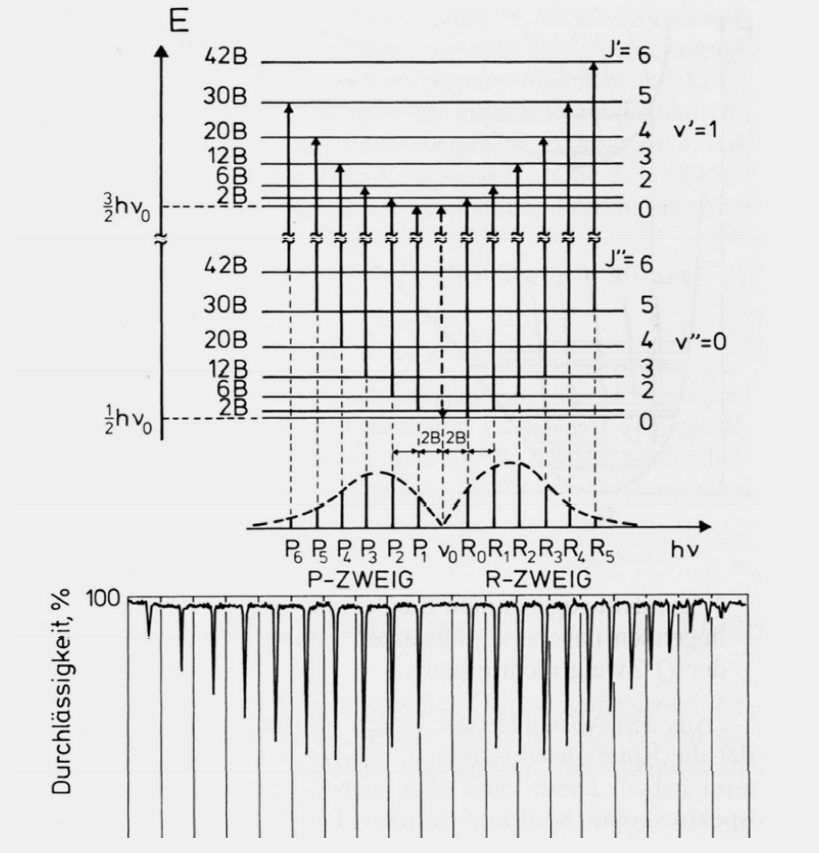
\includegraphics[width=\linewidth]{figures/vl09/vl09_rotationsschwingung_uebergaenge.png}
		\captionof{figure}{Erlaubte Übergänge $\Delta\nu=\pm1$, $\Delta J=\pm1$ im Rotationsschwingungsspektrum \cite{Haken_Wolf_2006}.}
		\label{fig:vl09_rotationsc_uebergaenge}
	\end{minipage}
	\hfill
	\begin{minipage}{0.35\linewidth}
		Aus den Abständen der Spektrallinien (vgl. \autoref{fig:vl09_rotationsc_uebergaenge}) gewinnt man $ 2B$ und somit Information über die Struktur des Moleküls. Aufgrund von $\mathrm{k}_{\mathrm{B}}T = \SI{200}{\centi \meter ^{-1}}$ bei Raumtemperatur und $ \mathrm{h} \nu_{\text{vib}} = \SI{1000}{ \centi \meter ^{-1}}$ ist $ \nu =1 $ fast immer thermisch unbesetzt und die Intensitäten in Absorbtionsspektren können durch die Entartung ( $2J +1$) gemeinsam mit dem Boltzmannfaktor bestimmt werden.
	\end{minipage}

	
